% -*- mode: noweb; noweb-default-code-mode: R-mode; -*-
\documentclass[a4paper]{article}


% \VignetteIndexEntry{An R Package for comparative analysis by independent contrasts} 
% \VignetteDepends{ape} 
% \VignetteKeyword{stats} 
% \VignetteKeyword{kwd2} 

\title{The CAIC package: comparative methods using independent contrasts}
\author{David Orme}




\usepackage{/Library/Frameworks/R.framework/Resources/share/texmf/Sweave}
\begin{document}

\maketitle

This document illustrates the use of the CAIC package for R (R Development Core Team, 2007) in carrying out comparative analyses using independent contrasts methods to account for phylogenetic autocorrelation. The CAIC package reimplements the methods originally implemented in the Mac Classic programs CAIC (Purvis and Rambaut, 1995) and MacroCAIC  (Agapow and Isaac, 2002) and this vignette draw heavily on the original manuals to those programs. The CAIC package, and the code in this vignette, requires the `ape' package (Paradis et al. 2004).

\section{Background}
Comparing the traits of species (or of groups of species of higher taxonomic rank) can produce deep insights into evolutionary processes. However, all such analyses should take into account the degree to which species are related and hence do not provide independent data on a hypothesis. This can lead both to situations in which apparently strong relationships rest on relatively few truly independent events (Fig. \ref{whyCAIC}a) or where strong relationships within groups are masked by phylogenetic differences between groups (Fig. \ref{whyCAIC}b). One way around this problem, originally described by Felsenstein (1985), is to recognize that the differences between taxa on either side of a bifurcating node represent independent evolutionary trajectories and that these differences (`independent contrasts') can be used to test hypotheses in a way that accounts for the phylogenetic autocorrelation between the taxa. Pagel (1992) extended this method to permit contrasts to be calculated at polytomies.

\begin{figure}[htbp]
  \begin{center}
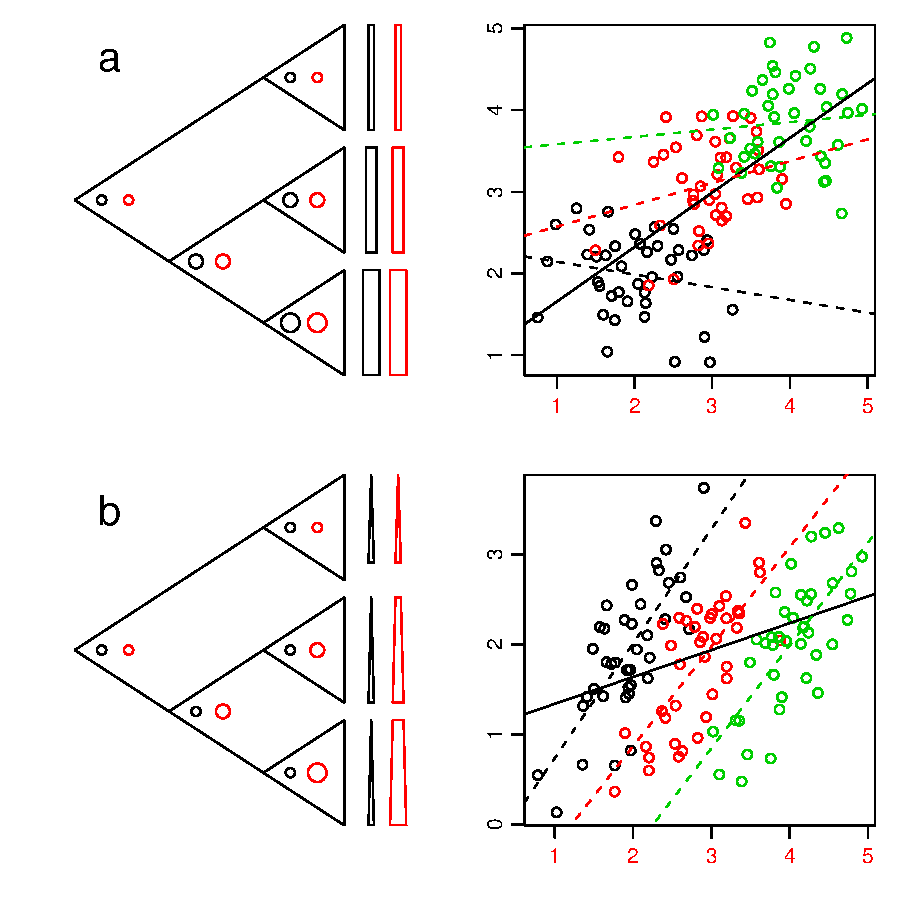
\includegraphics{caic-001}
    \caption{Phylogenetic autocorrelation in action. a) Simple regression (solid line) suggests a strong relationship between two variables; the phylogeny shows that within the three main groups, there is no consistent relationship (dashed lines) and the apparent relationship stems from only two linked shifts in the means of the traits early in the evolution of the clade. b) Simple regression (solid line) suggests a weak positive relationship between the two variables; the phylogeny shows that there are strong positive relationships between the traits within each of the three main groups but this is masked by early shifts in the mean value of the red trait.}
    \label{whyCAIC}
  \end{center}
\end{figure}



\section{Datasets}

The example in this document will make use of the following artificially generated datasets. In addition to being used in these examples, these datasets were also analyzed using the original programs and so  provide a benchmark test for the reimplemenation

\begin{description}
  \item[SmallTree] A dataset containing two phylogenies and two data frames. One phylogeny (diTree) is a 15 tip, fully bifurcating tree; three nodes in this phylogeny have been collapsed to give a second topology (polyTree) containing polytomies (Fig. \ref{smalltrees}). The data frames (SmallTreeDat and SmallTreeDatNA) contain data for each of the tips in the tree. They contain a column of tip names (tip), two continuous variables (weight and othervar), a column of the number of species in the tip group (nSpp) and two categorical variables (catX2 and catX3). SmallTreeDatNA differs only in having two tips for which no data is available.
  \item[BigTree] A dataset containing a larger phylogeny of 200 tip (BigTree) and a dataframe (BigTreeDat) providing four continuous variables (yv, xc1, xc2, xc3) and one binary categorical variable (xf) for each of the tips in the tree.
\end{description}


\begin{Schunk}
\begin{Sinput}
> library(ape)
> data(SmallTree)
> par(mfrow = c(2, 1))
> plot(diTree)
> plot(polyTree)
\end{Sinput}
\end{Schunk}
\begin{figure}[htbp]
  \begin{center}
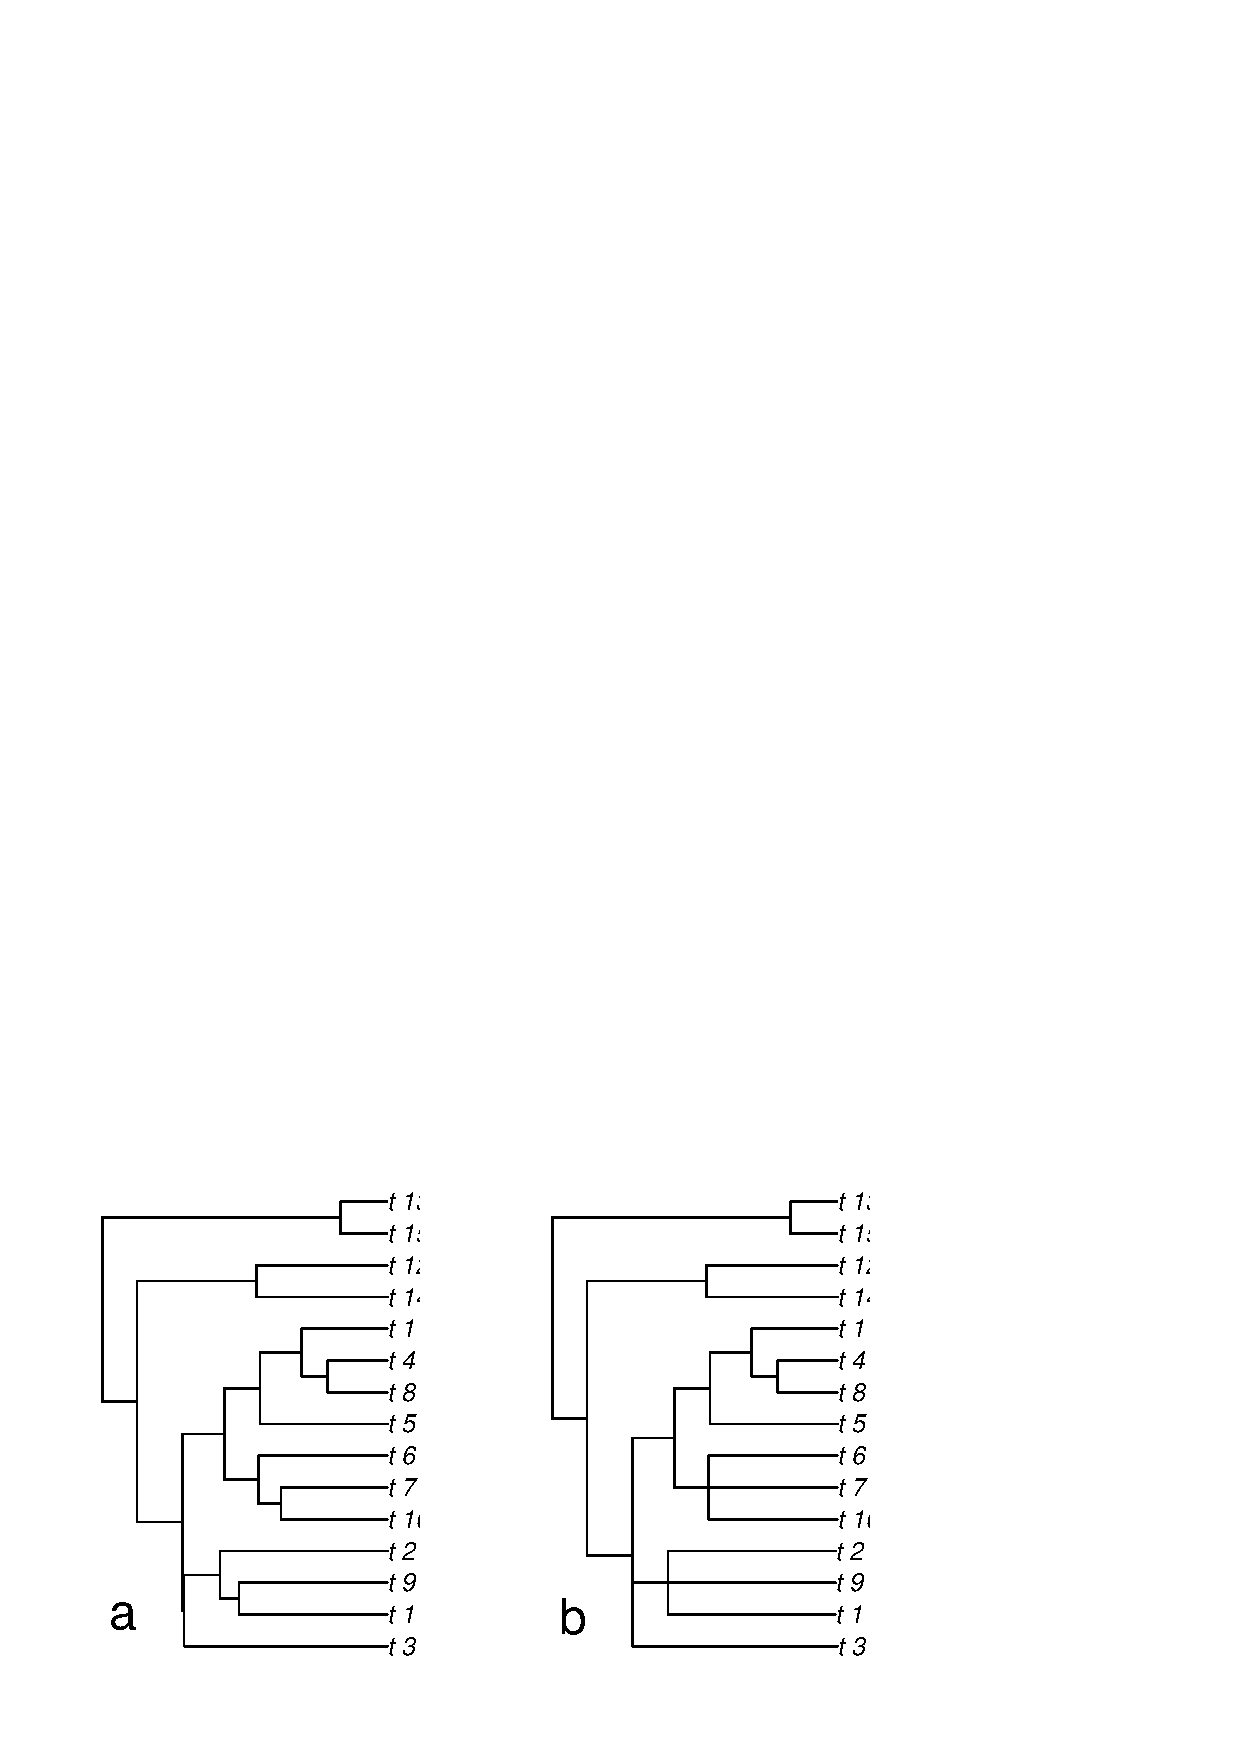
\includegraphics{caic-003}
    \caption{Phylogenies available in the smallTree dataset: a) diTree and b) polyTree.}
    \label{smalltrees}
  \end{center}
\end{figure}


\section{Analyses using the CAIC package.}

The CAIC package implements both CAIC and MacroCAIC analyses using a formula interface, as in the standard R \texttt{lm()} function. Both the \texttt{caic()} and \texttt{macrocaic()} functions need the user to provide a phylogeny (\texttt{phy}) and a data frame (\texttt{data}) containing trait data on the tips of the phylogeny. One column from the data frame (\texttt{names.col}) is used to match data between the tips of the phylogeny and the data frame; the matching process is done automatically by both functions. The phylogeny must be provided in the \texttt{phylo} structure provided by the ape package, which provides functions to read trees from newick, nexus and ape format files. In both functions, a reference variable (\texttt{ref.var}) may also be provided. This is required in order to standardize the directions in which contrasts are calculated in multivariate models. If no reference variable is provided, the function defaults to using the first explanatory variable specified in the model formula. 

\subsection{`Crunch' algorithm}


\subsection{`Brunch' algorithm}







\section{References}
Felsenstein, J.  (1985).  Phylogenies and the comparative method.  Am. Nat.  125, 1---15\\
Pagel, M. D. (1992). A method for the analysis of comparative data.  J. theor. Biol. 156, 431---442\\
Purvis, A. and Rambaut, A. (1995) Comparative analysis by independent contrasts (CAIC): an Apple Macintosh application for analysing comparative data.  Computer Appl. Biosciences 11, 247---251\\
Agapow, P.-M. and Isaac, N. J. B. (2002) MacroCAIC: correlates of species richness. Diversity \& Distributions, 8, 41---43\\
Paradis E., Claude J. and Strimmer K. 2004. APE: analyses of phylogenetics and evolution in the R language.  Bioinformatics 20, 289-290.\\
R Development Core Team (2007). R: A language and environment for statistical computing. R Foundation for  Statistical Computing, Vienna, Austria. ISBN 3-900051-07-0, URL http://www.R-project.org.\\



\end{document}
